\documentclass[letterpaper,dvipsnames]{article}
%\documentclass[12pt, letterpaper, twoside]{article}
% the default font size is 10pt
% letterpaper for US Letter
% a4paper for A4 (the standard in almost all the rest of the world)
% twocolumn, twoside

\usepackage{layout} % use \layout* to print the current details plus the layout shape

\usepackage{showframe} % To render a frame marking the margins 

\usepackage[utf8]{inputenc}

% epigraph for quote at start of section
\usepackage{epigraph}
\setlength\epigraphwidth{8cm}
\setlength\epigraphrule{0pt}
\renewcommand{\epigraphsize}{\small\itshape}

% \href{link}{name} or \url{link}
\usepackage{hyperref}

% to use colours
\usepackage{xcolor}

% Code formatting with the listing package is highly customizable.
\usepackage{listings}
 
\definecolor{codegreen}{rgb}{0,0.6,0}
\definecolor{codegray}{rgb}{0.5,0.5,0.5}
\definecolor{codepurple}{rgb}{0.58,0,0.82}
\definecolor{backcolour}{rgb}{0.95,0.95,0.92}

\lstdefinestyle{python-style}{
    backgroundcolor=\color{backcolour},   
    commentstyle=\color{codegreen},
    keywordstyle=\color{magenta},
    numberstyle=\tiny\color{codegray},
    stringstyle=\color{codepurple},
    basicstyle=\ttfamily\footnotesize,
    breakatwhitespace=false,         
    breaklines=true,                 
    captionpos=b,                    
    keepspaces=true,                 
    numbers=left,                    
    numbersep=5pt,                  
    showspaces=false,                
    showstringspaces=false,
    showtabs=false,                  
    tabsize=2
}

% to manage images
\usepackage{graphicx}
\graphicspath{ {./images/} }

\title{\LaTeX{} Experiments}

\author{AeAeA}

\begin{document}

\maketitle

%==============================================================================
\section{TeX distributions}

%--------------------------------------
\subsection{MacTeX}

The best for Mac.
\begin{verbatim}$ brew cask install mactex\end{verbatim}

%--------------------------------------
\subsection{Visual Studio Code LaTeX Workshop Extension}

LaTeX Workshop is an extension for Visual Studio Code, aiming 
to provide core features for LaTeX typesetting with Visual Studio Code.
\begin{itemize}
    \item \url{https://github.com/James-Yu/LaTeX-Workshop}
    \item \url{https://github.com/James-Yu/LaTeX-Workshop/wiki/Compile}
\end{itemize}
Build LaTeX file by calling the command \verb|Build LaTeX project| from the\\
Command Palette or from the TeX badge. This command is bound to \\
\verb|Cmd+Ctrl+b|

You can change VS Code settings by opening Settings tab:\\ 
\verb|Cmd+, -> Extensions -> LaTeX| \\ 
or, alternatively, by directly editing settings.json file:\\ 
\verb|~/Library/Application\ Support/Code/User/settings.json| \\
Recommended settings for LaTeX Workshop:
\begin{verbatim}
{
    "latex-workshop.view.pdf.viewer": "tab",
    "latex-workshop.latex.outDir": "%DIR%/texout",
    "latex-workshop.latex.autoBuild.run": "never",
    "latex-workshop.latex.autoClean.run": "onBuilt"
}
\end{verbatim}

%--------------------------------------
\subsection{MiKTeX}

Not for Mac. Old MiKTeX installation:\\
\verb+/usr/local/bin/+\\
\verb+/Applications/MiKTeX\ Console.app/+

%--------------------------------------
\subsection{TinyTeX}

TinyTeX - a lightweight, cross-platform, portable, and 
easy-to-maintain \LaTeX{} distribution based on TeX Live. 

Currently TinyTeX works best for R users. Installing and 
maintaining TinyTeX is easy for R users, since the R package 
tinytex has provided wrapper functions.

For other (non-R) users:
\begin{itemize}

    \item TinyTeX docs: \url{https://yihui.org/tinytex/}

    \item In the directory \\
          \verb|~/Library/TinyTeX/texmf-dist/tex/latex/| \\
          you can find all \LaTeX{} packages installed for TinyTeX.
    
    \item If you compile a LaTeX document and run into an error message 
          like this:\\
          \verb+! LaTeX Error: File `times.sty' not found.+ \\
          It basically indicates a missing LaTeX package.

          Use the command \verb+tlmgr search+ to find the name of 
          the missing package:\\
          \verb+$ tlmgr search --global --file "/times.sty"+\\
          \verb+psnfss: texmf-dist/tex/latex/psnfss/times.sty+

          In this case, the missing package is \verb+psnfss+, and we 
          can install a package via \verb+tlmgr install+, e.g., \\
          \verb+$ tlmgr install psnfss+

          If you still see error messages that you don’t understand, 
          you may need to update everything:\\
          \verb+$ tlmgr update --self --all+\\
          \verb+$ tlmgr path add+\\
          \verb+$ fmtutil-sys --all+
    
    \item To uninstall TinyTeX use command line:\\
          \verb+$ tlmgr path remove+\\
          \verb+$ rm -r "~/Library/TinyTeX"+
          
\end{itemize}


%==============================================================================
\section{Epigraph}

\epigraph
{In doing what we ought we deserve no praise, because it is our duty.}
{--- \textup{Saint Augustine}}

%--------------------------------------
\subsection{Online docs}
\begin{itemize}
    \item \url{https://en.wikibooks.org/wiki/LaTeX} 
          \LaTeX wiki (very informative).
    \item \url{http://texdoc.net/} TeXdoc is a \TeX and \LaTeX
          documentation lookup system.
\end{itemize}

%--------------------------------------
\subsection{Using colours}
 
This example shows different examples on how to use the \texttt{xcolor} package 
to change the colour of elements in \LaTeX.
 
\begin{itemize}
\color{blue}
    \item blue
\color{cyan}
    \item cyan
\color{ForestGreen}
    \item ForestGreen
\color{RubineRed}
    \item RubineRed
\end{itemize}
 
\begin{flushleft} \color{red} \rule{\linewidth}{1pt} \end{flushleft}

Change the text color to \textcolor{red}{red}, or the background color to 
\colorbox{BurntOrange}{BurntOrange}.

%--------------------------------------
\subsection{Units and page layout}
\begin{itemize}
    \item \url{https://en.wikibooks.org/wiki/LaTeX/Page_Layout}
\end{itemize}
Standard \LaTeX units: mm, cm, pt, in, with $1in = 72.27pt$ and 
$1pt = 0.3515mm$ and $1mm = 2.8445pt$. \\
US Letter (letterpaper) is 8.5 x 11 in, 215.9 x 279.4 mm, 
614.295 x 794.97 pt, aspect ratio 1.294. \\
A4 (a4paper) is 8.3 x 11.7 in, 210 x 297 mm, 597.44 x 844.95 pt, aspect ratio 1.414 
($\approx\sqrt{2}$).

\newpage

\marginpar{Margin note\\ 
1in=72.27pt\\ 
1pt=0.35mm\\ 
1mm=2.84pt\\
\\
textwidth\\ 
345pt = 4.77in = 121.48mm\\
\\
textheight\\
550pt = 7.61in = 193.66mm
} 
The current page layout picture below is generated by calling command\\ 
\verb+\layout*+ from \verb+\usepackage{layout}+.\footnote{An example footnote.} 

\vspace{5mm}

\layout*

\newpage

%==============================================================================
\section{verbatim and listings}

%--------------------------------------
\subsection{verbatim}
\begin{verbatim}
Text enclosed inside 
    \begin{verbatim} ... \end {verbatim} 
environment                      is printed directly 
and all \LaTeX{} commands are ignored.
\end{verbatim}

\begin{verbatim*}
Text enclosed inside \begin{verbatim*} environment 
    is printed directly 
and all \LaTeX{} commands are ignored,
and white spaces are emphasized with a special symbol.
\end{verbatim*}

Use \verb| \verb+<inline verbatim text>+ | like this:\\
The \verb+\ldots+ command produces \ldots

%--------------------------------------
\subsection{listings: Source code printing}
\begin{itemize}
    \item \href
    {http://texdoc.net/texmf-dist/doc/latex/listings/listings.pdf}
    {listings} package documentation
    \item \url{https://www.overleaf.com/learn/latex/Code_listing}
\end{itemize}

%--------------------------------------
\subsubsection{minimal setup}

Example of using the \verb+\begin{lstlisting}[language=Python]+ 
environment \\
from the \verb+\usepackage{listings}+ package to highlight Python code:

\begin{lstlisting}[language=Python]
import numpy as np
    
def incmatrix(genl1,genl2):
    m = len(genl1)
    n = len(genl2)
    M = None #to become the incidence matrix
    VT = np.zeros((n*m,1), int)  #dummy variable
    
    #compute the bitwise xor matrix
    M1 = bitxormatrix(genl1)
    M2 = np.triu(bitxormatrix(genl2),1) 
    
    for i in range(m-1):
        for j in range(i+1, m):
            [r,c] = np.where(M2 == M1[i,j])
            for k in range(len(r)):
                VT[(i)*n + r[k]] = 1;
                VT[(i)*n + c[k]] = 1;
                VT[(j)*n + r[k]] = 1;
                VT[(j)*n + c[k]] = 1;
    
                if M is None:
                    M = np.copy(VT)
                else:
                    M = np.concatenate((M, VT), 1)
    
                VT = np.zeros((n*m,1), int)
    
    return M
\end{lstlisting}

%--------------------------------------
\subsubsection{with code styles and colours}

You need \verb+\usepackage{xcolor}+ package for the code colouring. \\
Just like in floats (tables and figures), captions can be added to a 
listing for a more clear presentation. This caption can be later used 
in the list of Listings \verb+\lstlistoflistings+.

\lstset{style=python-style}
\begin{lstlisting}[language=Python, caption=Python example]
import numpy as np
    
def incmatrix(genl1,genl2):
    m = len(genl1)
    n = len(genl2)
    M = None #to become the incidence matrix
    VT = np.zeros((n*m,1), int)  #dummy variable

    s = "codepurple"
    
    #compute the bitwise xor matrix
    M1 = bitxormatrix(genl1)
    M2 = np.triu(bitxormatrix(genl2),1) 
    
    for i in range(m-1):
        for j in range(i+1, m):
            [r,c] = np.where(M2 == M1[i,j])
            for k in range(len(r)):
                VT[(i)*n + r[k]] = 1;
                VT[(i)*n + c[k]] = 1;
                VT[(j)*n + r[k]] = 1;
                VT[(j)*n + c[k]] = 1;
    
                if M is None:
                    M = np.copy(VT)
                else:
                    M = np.concatenate((M, VT), 1)
    
                VT = np.zeros((n*m,1), int)
    
    return M
\end{lstlisting}

\newpage

%==============================================================================
\section{Inserting Images}
\LaTeX can not manage images by itself, so we need to use the graphicx package. 
To use it, we include the following line in the preamble: 
\verb+\usepackage{graphicx}+

The command \verb+\graphicspath{ {./images/} }+ tells \LaTeX that the images 
are kept in a folder named images under the directory of the main document.

\begin{figure}[h]
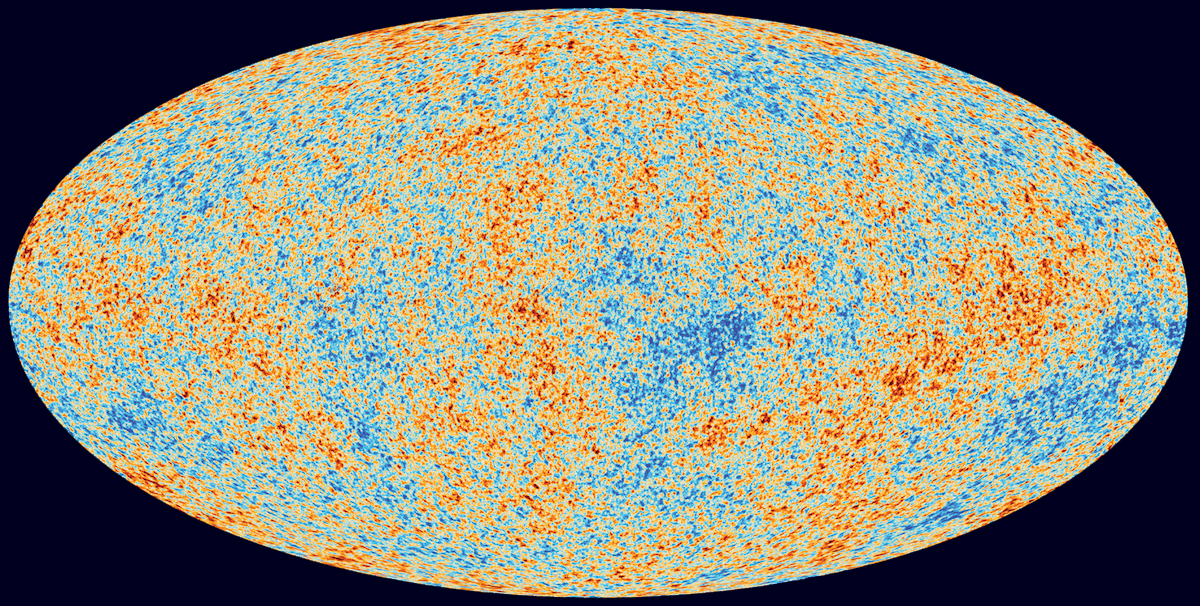
\includegraphics[width=\textwidth]{cosmic-microwave-background}
\caption{Cosmic Microwave Background, by Planck Space Telescope}
\end{figure}

\newpage

\lstlistoflistings

\listoffigures

\end{document}